% !TEX root = diplomarbeit.tex
\chapter{Elektronik}
\renewcommand{\kapitelautor}{Autor: Lucas Ullrich}

%%%%%%%%%%%%%%%%%%%%%%%%%%%%%%%%%%%%%%%%%%%%%%%%%%%%%%%%%%%%%%%%%%%%%%%%%%%%%%%
\section{Allgemeine technische Planung}
Für die Umsetzung eines autonomen Fluges sind diverse Sensoren sowie eine entsprechende Auswertung der gelieferten Daten notwendig.
Alle Daten müssen an einem zentralen Ort für eine Auswertung zusammenlaufen, aus diesen können schließlich die notwendigen Flugparameter ermittelt werden.

  \subsection{Benötigte Elemente}
  Eine eigens entwickelte Ansteuerung der einzelnen Rotoren gestaltet sich als sehr umfangreich, deshalb wird ein fertiger Flight-Controller verwendet.
  Das System selbst basiert auf einer Modulbauweise, so können einzelne Komponenten, je nach Bedarf, inkludiert oder exkludiert werden.
  Sämtliche Informationen werden über einen PIC-Mikrocontroller geleitet und über diesen ausgewertet.

    \subsubsection{PIC}
    Als zentrale Recheneinheit wird ein PIC18F46K22 verwendet. Dieser bietet ausreichend viel Speicherplatz und Pins für eine Testphase und kann mit einer Geschwindigkeit
    von bis zu $\SI{64}{\mega\hertz}$ intern getaktet werden. So ist keine aufwändige Oszillator-Schaltung notwendig und es ist eine vernünftig hohe Geschwindigkeit bei der
    Auswertung erzielbar.

    Der PIC ist dabei für die Auswertung der Kamera, des Ultraschallsensors, des Fernsteuerungsempfängers AR610 von Spektrum sowie dem WLAN-Modul zuständig.
    Je nach gewähltem Flugmodus steuert der PIC einen Multiplexer so an, dass ein autonomer oder manueller Flug möglich ist.
    Außerdem werden von ihm die Servo-Impulse für den Flightcontroller ausgegeben.

    \subsubsection{DJI NAZA-M lite, Flamewheel F550}
    Der Flightcontroller NAZA-M lite von DJI ist ein bereits mit dem Flamewheel F550 ARF-Kit (Almost Ready to Fly) verkaufter Flugregler.
    Er ist dafür zuständig, dass die ankommenden Steuerimpulse namens Aileron, Elevator, Throttle und Rudder richtig verarbeitet werden.
    Dabei findet bereits eine automatische Regelung der Fluglage statt, der Hexacopter neigt sich also nicht \zB über einen Winkel von $\SI{45}{\degree}$.
    Ebenso werden die einzelnen Rotoren bereits so angesteuert, dass hier kein externer Eingriff mehr notwendig ist.
    \begin{figure}[H]
      \begin{centering}
        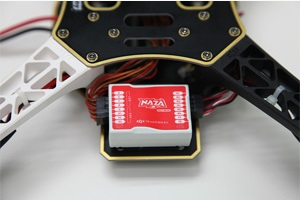
\includegraphics[width = 0.6\textwidth]{Bilder/NAZA_M-lite}
      \par\end{centering}
      \caption[Flightcontroller DJI NAZA-M lite]{Flightcontroller DJI NAZA-M lite\cite{NAZA_M-lite}}
      \label{NAZA_M-lite}
    \end{figure}

    \subsubsection{WLAN}
    Das WLAN-Modul RN171 von welches von Microchip verkauft wird bietet die Schnittstelle zwischen Server und Hexacopter. Die Daten können entweder vom Server gesendet
    und vom PIC empfangen werden oder umgekehrt.
    Das WLAM-Modul wird mit einer UART-Schnittstelle betrieben. Für eine Kommunikation sind also nur 2 Leitungen notwendig.
    Es bietet die Möglichkeit über eine Anwendung wie TeraTerm oder HTerm eingestellt zu werden, zusätzlich wird aber auch ein Webinterface angeboten, dieses muss jedoch zuvor
    aktiviert werden.

    \begin{figure}[tbh]
      \begin{centering}
        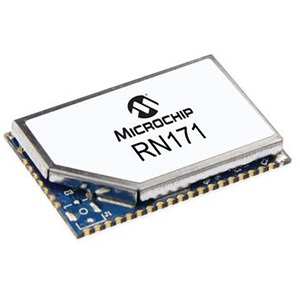
\includegraphics[width = 0.5\textwidth]{Bilder/RN171}
      \par\end{centering}
      \caption[WLAN-Modul RN171]{WLAN-Modul RN171\cite{RN171}}
      \label{RN171}
    \end{figure}

    Die Datenübertragung findet dabei für den Nutzer sehr unproblematisch dar. Einerseits sind konfigurierbare Pins vorhanden um die Verbindung zu steuern und zu überwachen,
    andererseits braucht man sich nicht mehr um das Verpacken der Datenpakete kümmern.

%%%%%%%%%%%%%%%%%%%%%%%%%%%%%%%%%%%%%%%%%%%%%%%%%%%%%%%%%%%%%%%%%%%%%%%%%%%%%%%
\section{Blockschaltbild}
Die einzelnen Komponenten werden über den Mikrocontroller vereint. Sämtliche Berechnungen und Auswertung finden auf diesem statt und werden über diesen ausgegeben \bzw
weitergeleitet. Der Flightcontroller NAZA-M lite wird an die A, E, R und T Pins angeschlossen.
\begin{figure}[H]
  \begin{centering}
    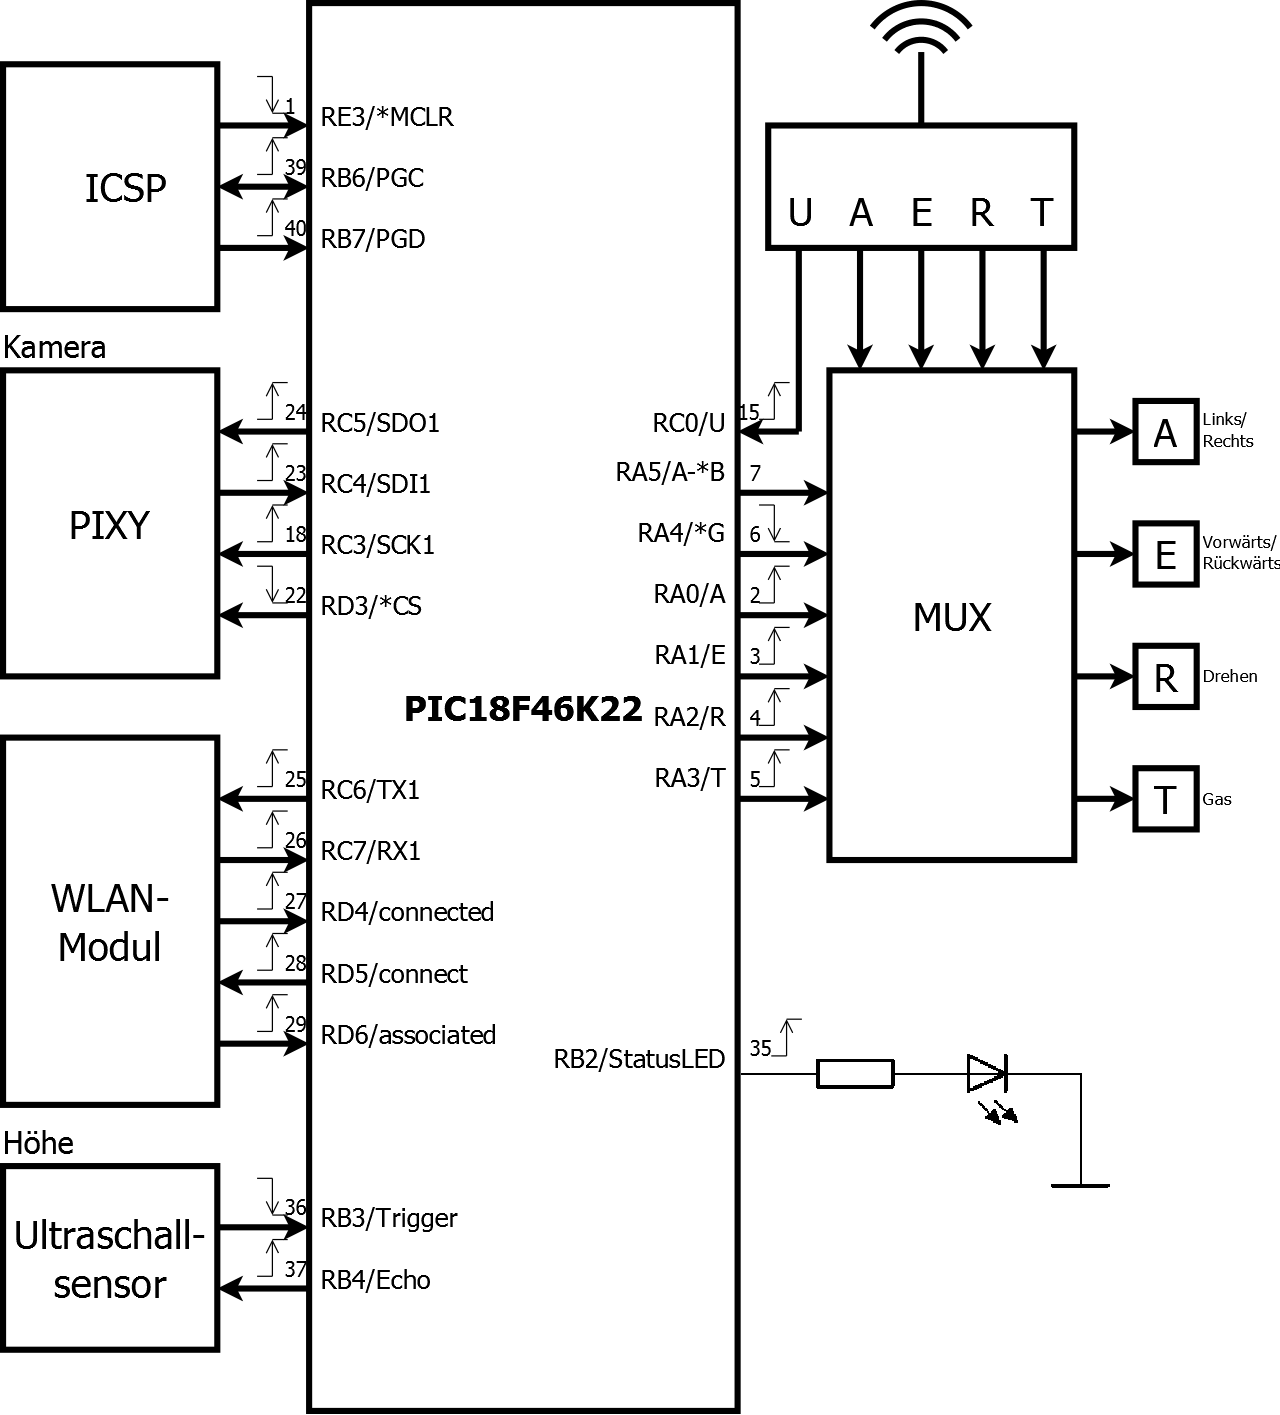
\includegraphics[width = 1\textwidth]{Bilder/Blockschaltbild}
  \par\end{centering}
  \caption{Blockschaltbild der Hauptplatine}
  \label{Blockschaltbild}
\end{figure}

  \subsection{Hauptplatine}
  Die Hauptplatine dient als zentrales Kommunikationselement. Auf dieser befindet sich der PIC welcher für sämtliche Berechnungen und Auswertungen zuständig ist.
  Um ein ausreichendes Maß an Kommunikationsfähigkeit zu ermöglichen befinden sich auf ihr folgende Anschlüsse:
  \begin{itemize}
    \item $+\SI{5}{\volt}$ Spannungsversorgung
    \item Eingänge des Fernsteuerungsempfängers (5 Pins)
    \item Ausgänge zum Flightcontroller (4 Pins)
    \item Anschluss für den Ultraschallsensor
    \item Anschluss für die PIXY CMUcam5
    \item Anschluss für das WLAN-Modul
  \end{itemize}

    \subsubsection{Technische Planung}
    Das Hauptkriterium für die Hauptplatine war es alle notwendigen Komponenten für einen autonomen Flug zu enthalten. Wichtig waren hier vor allem die Kamera,
    der Ultraschallsensor sowie die Möglichkeit auf einen manuellen Flug zu wechseln.

    \subsubsection{Umsetzung}
    Für die Umsetzung wurden die einzelnen Komponenten entsprechend ihrer Funktion im Schalplan verbunden und aus diesem ein Platinen-Layout erstellt.
    Das Platinen-Layout wurde schließlich mit einem Fräsplotter auf das Rohmaterial übertragen.

    \begin{figure}[tbh]
      \begin{centering}
        \subfigure[Oberseite]{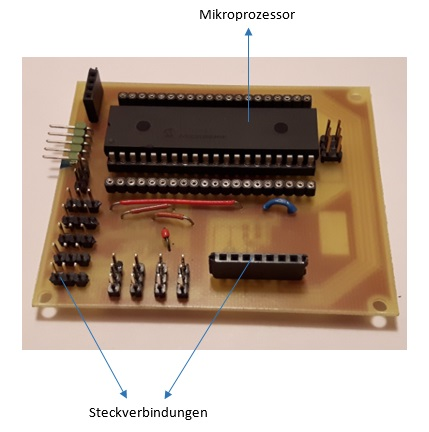
\includegraphics[width = 0.49\textwidth]{Bilder/HP_top}}
        \subfigure[Unterseite]{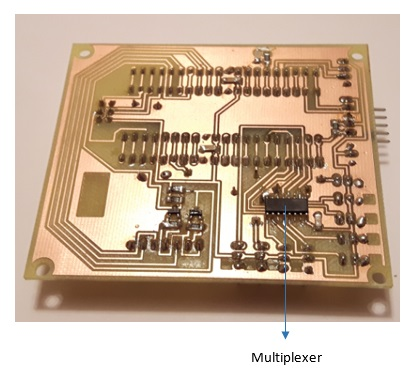
\includegraphics[width = 0.49\textwidth]{Bilder/HP_bot}}
      \par\end{centering}
      \caption{Die bestückte Hauptplatine}
      \label{Hauptplatine}
    \end{figure}

    \subsubsection{Herausforderungen und Lösungen}
    Eine Herausforderung stellte die geringe Deckkraft des schwarzen Toners beim ätzen der Platine dar. Durch zu wenig Toner auf der Belichtungsvorlage sind
    angeätzte Masseflächen entstanden. Um dennoch eine ordentliche Platine zu haben wurde diese schließlich gefräst. Dies hat auch viel Arbeit beim Bohren der
    Löcher erspart.

  \subsection{WLAN-Modul}
  Das WLAN-Modul dient als Schnittstelle zwischen Hauptplatine und Server. Auf dieser Platine befinden sich das WLAN-Modul RN171 sowie ein Spannungsregler und Level-Shifter
  um eine Kompatibilität mit den anderen Komponenten zu gewährleisten.

    \subsubsection{Technische Planung}
    In der Planung war die Versorungsspannung des WLAN-Modul das Hauptaugenmerk. Für den Betrieb sind $\SI{3.3}{\volt}$ notwendig, eine $\SI{5}{\volt}$ Toleranz ist nicht gegeben.
    Aufgrund der fehlenden Toleranz müssen alle Leitungen die zur Kommunikation dienen entweder auf $\SI{5}{\volt}$ angehoben oder auf $\SI{3.3}{\volt}$ abgesenkt werden,
    andernfalls kann es zu Datenverlust oder sogar einer Beschädigung eines Moduls kommen.

    \subsubsection{Umsetzung}

    \subsubsection{Herausforderungen und Lösungen}
